\documentclass[11pt]{article}
\usepackage{graphicx}
\usepackage[margin=1in]{geometry}
%Gummi|065|=)
\begin{document}
\textbf{Doug Woodward}

Data Set: Flags

Data Completeness: 100\%

Instances: 194

Attributes: 30

\begin{center}
\begin{tabular} { | c | c | c |}
\hline
Attribute & Type & Note \\ [0.5ex] 
\hline\hline
name & Nominal & \\
landmass & Categorical & Continents \\
zone & Categorical & Geo Quadrant \\
area & Numerical &  Size of Country \\
population & Numerical &  \\
language & Categorical &  Most languages under "Other" \\
religion & Categorical &   \\
bars & Numerical &  Vertical Bars \\
stripes & Numerical &  Horizontal Stripes \\
colours & Categorical &   \\
red & Categorical(Binary) &  \\
green & Categorical(Binary) &  \\
blue & Categorical(Binary) &  \\
gold & Categorical(Binary) &  Includes Yellow \\
white& Categorical(Binary) &  \\
black & Categorical(Binary) &  \\
orange & Categorical(Binary) &  Includes Brown \\
mainhue & Categorical &  Most dominant colour in flag \\
circles & Numerical &  \\
crosses & Numerical &  \\
saltires & Numerical &  \\
quarters & Numerical &  \\
sunstars & Numerical &  \\
crescent & Categorical(Binary)  &  \\
triangle & Categorical(Binary)  &  \\
icon & Categorical(Binary)  &  Any inanimate images(ie Boat) \\
animate &  &  Any animate image (Living thing) \\
text & Categorical(Binary)  &  \\
topleft & - &  Colour in top left \\
botright & - &  Colour in bottom left? \\
\hline
\end{tabular}
\end{center}

\textbf{Analysis:}
	The most commonly occurring color is Red(153) followed by White(146). The least common color(s) are Orange/Brown. \\
	
	Some simple clustering on only color related attributes yields an expected Red/Blue Split.\\
	
	The crescent symbol is used by not only Muslim countries, but also by Buddhist and Hindu countries as well.\\
	
	The Top Left and Bottom Right(may be bottom left) attributes are fairly similar, indicating that most flags do not use vertical\\ gradients or sections.
	
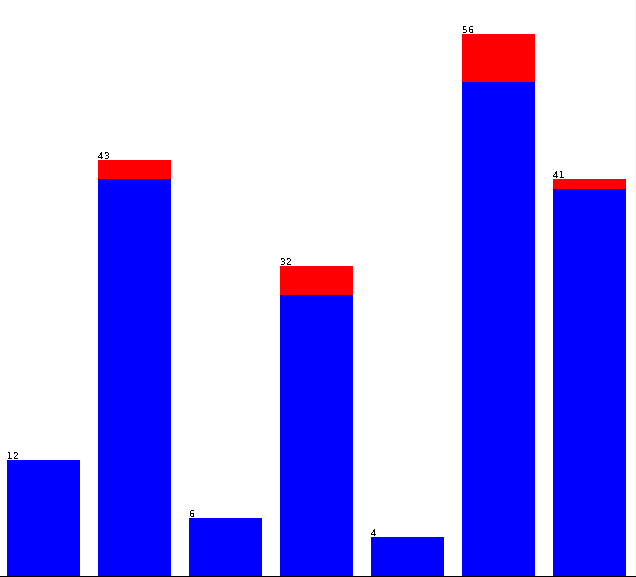
\includegraphics[scale=.2]{topleft} 
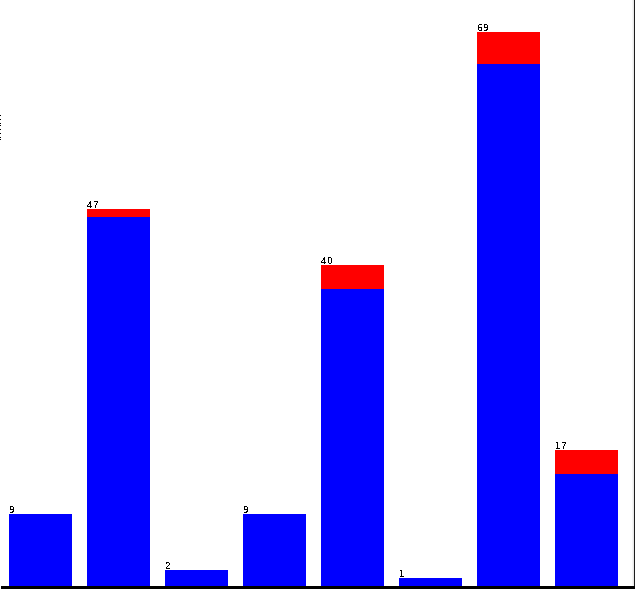
\includegraphics[scale=.2]{botright} \\

Additionally, the frequency of an animate object (39) or an inanimate icon (49) is roughly the same.\\

\textbf{Outliers:}
	
	Some Outliers in size, but that is not of interest here, indeed, the data for size, quadrant, population, and a few others could be thrown away for a purely vexilogical study. Because the majority of attributes here are categorical, defining an outlier is difficult and subjective to the analysis being run.
	
\textbf{Notes:}
	Data is labeled, but not particularly well.
	

\end{document}
